% ============================================================
% ESPOL - FIEC - SOFG1007 Ingeniería de Software I
% Plantilla LaTeX - Especificación de Proyecto FINAL (2do parcial)
% ============================================================
% Cómo usar esta plantilla:
%   1. Reemplace todos los textos entre corchetes [así] con la
%      información real de su proyecto.
%   2. Coloque el logo de ESPOL en imagenes/logo_espol.png
%      (si no existe, se muestra una caja de reemplazo y el
%      documento compila igual).
%   3. Cada diagrama UML tiene una "caja de reemplazo" que debe
%      sustituirse por \includegraphics{...} apuntando a la
%      imagen real exportada desde su herramienta de modelado
%      (indique el nombre de la herramienta donde se solicita).
%   4. Compile con pdflatex (2 veces) o latexmk -pdf main.tex
% ============================================================

\documentclass[12pt,a4paper]{report}

% ---------------- Idioma y codificación ----------------
\usepackage[utf8]{inputenc}
\usepackage[T1]{fontenc}
\usepackage[spanish,es-tabla]{babel}
\spanishdecimal{.}

% ---------------- Página y geometría ----------------
\usepackage[margin=2.5cm,headheight=28pt]{geometry}
\usepackage{setspace}
\onehalfspacing

% ---------------- Gráficos y figuras ----------------
\usepackage{graphicx}
\usepackage{float}
\usepackage{caption}
\usepackage{subcaption}
\usepackage{pgffor}      % para \foreach (usado en los 32 diagramas de secuencia)

% ---------------- Tablas ----------------
\usepackage{array}
\usepackage{booktabs}
\usepackage{longtable}
\usepackage{tabularx}
\usepackage{multirow}
\usepackage{colortbl}

% Tipos de columna con centrado vertical (requiere \usepackage{array}):
% M{ancho} = centrado horizontal y vertical (para valores cortos: IDs, categorías, estados, etc.)
% L{ancho} = alineado a la izquierda y centrado vertical (para texto largo/párrafos)
\newcolumntype{M}[1]{>{\centering\arraybackslash}m{#1}}
\newcolumntype{L}[1]{>{\raggedright\arraybackslash}m{#1}}

% ---------------- Color, listas, enlaces ----------------
\usepackage[table]{xcolor}
\usepackage{enumitem}
\usepackage{pdfpages}     % para anexar el acta de conformidad escaneada (PDF)
\usepackage{underscore}   % permite usar "_" literal en nombres de archivo fuera de modo matemático
\usepackage{hyperref}
\usepackage{fancyhdr}
\usepackage{titlesec}
\usepackage{lastpage}

% ---------------- Colores institucionales (ajustar si se desea) ----------------
\definecolor{espolblue}{RGB}{0,51,102}
\definecolor{cajagris}{RGB}{245,245,245}

% ---------------- Colores del mapa de calor de riesgos (matriz 5x5) ----------------
\definecolor{riskmuybajo}{RGB}{198,239,206}
\definecolor{riskbajo}{RGB}{221,235,148}
\definecolor{riskmedio}{RGB}{255,230,153}
\definecolor{riskalto}{RGB}{255,192,120}
\definecolor{riskmuyalto}{RGB}{255,150,113}
\definecolor{riskextremo}{RGB}{237,108,108}

% ---------------- Colores de trazabilidad de diagramas (Heredado / Nuevo) ----------------
% Mismos tonos usados en el skinparam de los .puml (recursos/diagramas_uml/) para
% mantener consistencia visual entre el diagrama y su tabla de trazabilidad.
\definecolor{heredadobg}{RGB}{214,234,248}
\definecolor{nuevobg}{RGB}{213,245,227}

\hypersetup{
    colorlinks=true,
    linkcolor=espolblue,
    citecolor=espolblue,
    urlcolor=espolblue,
    pdftitle={Leodega - Especificación de Proyecto},
    pdfauthor={Darwin Leonardo Diaz Gonzalez; Geovanny Jahir Diaz Loor; Carla Alejandra Gutierrez Cordova; Johao Carlos Dorado Quinde},
    pdfsubject={SOFG1007 - Ingeniería de Software I - ESPOL},
}

% ---------------- Nombres en español (ajustes) ----------------
\addto\captionsspanish{%
  \renewcommand{\tablename}{Tabla}
  \renewcommand{\listtablename}{Índice de Tablas}
  \renewcommand{\listfigurename}{Índice de Figuras}
  \renewcommand{\contentsname}{Tabla de Contenido}
  \renewcommand{\appendixname}{Anexo}
  \renewcommand{\bibname}{Referencias}
}

% ---------------- Encabezado / pie de página ----------------
\pagestyle{fancy}
\fancyhf{}
\renewcommand{\headrulewidth}{0.4pt}
\lhead{\small ESPOL - FIEC - SOFG1007}
\rhead{\small Leodega}
\rfoot{\small Página \thepage\ de \pageref{LastPage}}
\lfoot{\small Ingeniería de Software I}

% ---------------- Estilo de capítulos ----------------
\titleformat{\chapter}[display]
  {\normalfont\bfseries\Large\color{espolblue}}
  {\chaptertitlename\ \thechapter}{10pt}{\Huge}
\titlespacing*{\chapter}{0pt}{-20pt}{20pt}

% ============================================================
% COMANDOS REUTILIZABLES PARA DIAGRAMAS UML
% ============================================================
% Caja de reemplazo (usar mientras no se tenga la imagen final).
% Cuando tenga la imagen exportada, reemplace el contenido de
% \DiagramaImagen por \includegraphics[width=0.9\textwidth]{ruta}
\newcommand{\DiagramaImagen}[3]{%
  % #1 = ancho relativo del \textwidth, #2 = alto relativo del \textheight, #3 = texto de la caja
  \IfFileExists{#3}{%
    \includegraphics[width=#1\textwidth,height=#2\textheight,keepaspectratio]{#3}%
  }{%
    \fbox{\begin{minipage}[c][#2\textheight][c]{#1\textwidth}%
      \centering\itshape\color{gray} Insertar aquí el diagrama:\\ \texttt{#3}
    \end{minipage}}%
  }%
}

% Genera una subsección con un diagrama a página completa, su
% descripción y la herramienta utilizada. Uso:
% \DiagramaPagina{Título del diagrama}{ruta/archivo.png}{etiqueta}{Descripción}
\newcommand{\DiagramaPagina}[4]{%
  \subsection{#1}
  \begin{figure}[H]
    \centering
    \DiagramaImagen{0.95}{0.55}{#2}
    \caption{#1}
    \label{fig:#3}
  \end{figure}
  \noindent\textbf{Descripción:} #4\par
  \bigskip
  \noindent\textbf{Herramienta de modelado utilizada:} \textit{[Ej. Visual Paradigm, StarUML, Draw.io]}
  \clearpage
}

\begin{document}

% ---------------- Portada ----------------
% ============================================================
% PORTADA
% ============================================================
\begin{titlepage}
\thispagestyle{empty}
\begin{center}

% --- Logo ESPOL ---
\IfFileExists{imagenes/logo-espol.jpg}{%
    
\includegraphics[width=14cm]{imagenes/logo-espol.jpg}
}{%
    \fbox{\begin{minipage}[c][3cm][c]{5cm}\centering [LOGO ESPOL]\end{minipage}}
}

\vspace{0.5cm}
{\large \textbf{ESCUELA SUPERIOR POLITÉCNICA DEL LITORAL}}\\[4pt]
{\large \textbf{FACULTAD DE INGENIERÍA EN ELECTRICIDAD Y COMPUTACIÓN}}\\[4pt]
{\large SOFG1007 -- INGENIERÍA DE SOFTWARE I}

\vspace{2cm}
{\Large \textbf{ESPECIFICACIÓN DE PROYECTO FINAL}}\\[6pt]
{\large Segundo Parcial}

\vspace{1.5cm}
\begin{center}
    {\Huge \textbf{LEODEGA}}\\[10pt]
    {\large\itshape Storage Marketplace}
\end{center}

\vspace{2cm}
\begin{minipage}{0.75\textwidth}
\centering
\textbf{Integrantes del equipo:}
\begin{tabularx}{\textwidth}{|l|X|c|}
\hline
\rowcolor{cajagris}
\textbf{No.} & \textbf{Nombre completo} & \textbf{Matrícula} \\
\hline
1 & Darwin Leonardo Díaz González & [ID] \\ \hline
2 & Geovanny Jahir Díaz Loor & [ID] \\ \hline
3 & Carla Alejandra Gutiérrez Córdova & [ID] \\ \hline
4 & Johao Carlos Dorado Quinde & [ID] \\ \hline
\end{tabularx}
\end{minipage}

\vspace{1.5cm}
\textbf{Profesor:} Mgti. Vanessa Jurado Alexandra Vite\\
\textbf{Cliente / Representante:} Leonardo

\vspace{1.5cm}
\textbf{Período académico:} PAO II -- 2026\\
\today

\end{center}
\end{titlepage}
\clearpage


% ---------------- Acta de conformidad del cliente (OBLIGATORIA) ----------------
\chapter*{Acta de Conformidad del Cliente}
\addcontentsline{toc}{chapter}{Acta de Conformidad del Cliente}
\thispagestyle{empty}
\noindent\textbf{Importante:} La ausencia de esta acta firmada implica una penalidad de -100 según la rúbrica de calificación. Adjunte el documento escaneado/firmado.

\bigskip
\IfFileExists{imagenes/acta_conformidad.pdf}{%
  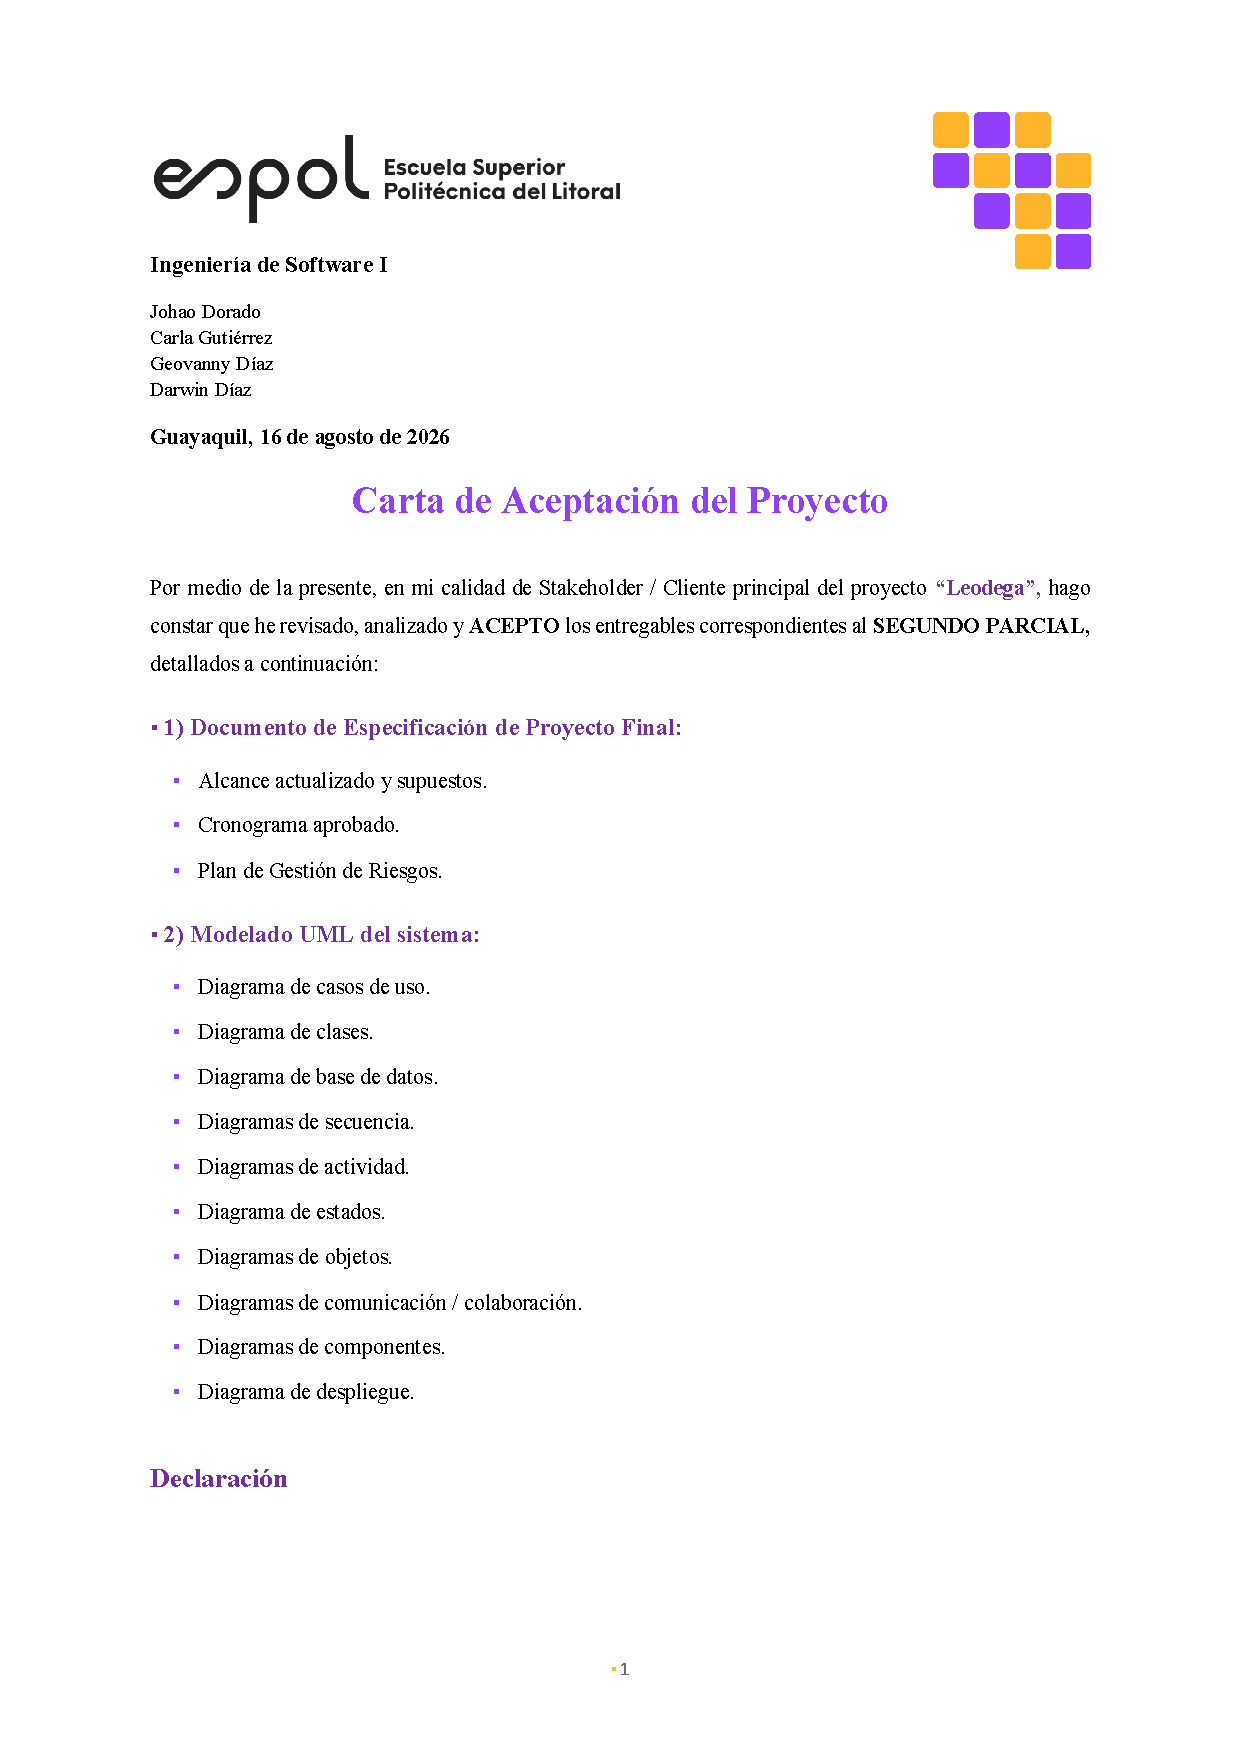
\includepdf[pages=-]{imagenes/acta_conformidad.pdf}
}{%
  \begin{center}
  \fbox{\begin{minipage}[c][0.6\textheight][c]{0.9\textwidth}
    \centering\itshape\color{gray}
    Insertar aquí el acta de conformidad firmada por el representante del cliente.\\
    (Reemplazar por: \texttt{imagenes/acta\_conformidad.pdf} usando \texttt{includepdf}, \\
    o insertar una imagen escaneada con \texttt{includegraphics})
  \end{minipage}}
  \end{center}
}
\clearpage

% ---------------- Índices ----------------
\tableofcontents
\clearpage
\listoffigures
\clearpage
\listoftables
\clearpage

% ---------------- Información general del proyecto ----------------
% ============================================================
% INFORMACIÓN GENERAL DEL PROYECTO
% Fuente: recursos/informacion_general/proyecto1P.tex
% (Documento de Especificación de Requerimientos, 1er parcial)
% ============================================================
\chapter{Información General del Proyecto}

\section{Descripción General}

\textbf{Leodega} es un \textit{marketplace} colaborativo de espacios de almacenamiento que conecta a propietarios de espacios ---arrendadores, en adelante \textbf{Storage Managers}--- con personas y organizaciones que necesitan almacenar sus bienes ---arrendatarios, en adelante \textbf{Clientes}---, bajo la supervisión de un \textbf{Administrador} del sistema. El proyecto parte de una plataforma web \textit{full-stack} ya existente, desarrollada bajo metodología Scrum, la cual se encontraba en fase de integración y pruebas al momento de ser entregada al equipo como punto de partida.

La plataforma heredada está construida sobre la siguiente base tecnológica:
\begin{itemize}[leftmargin=*]
    \item \textbf{Backend:} Laravel 12 (PHP 8.2+), autenticación basada en tokens con Laravel Sanctum, ORM Eloquent y base de datos PostgreSQL en producción (SQLite en desarrollo local), contenerizada con Docker Compose y desplegable en Railway.
    \item \textbf{Frontend:} React 19 con TypeScript y Vite, React Router DOM con rutas protegidas por rol, Tailwind CSS, Axios con interceptor de token Bearer, mapas con Leaflet/React-Leaflet, e internacionalización con i18next; desplegable en Vercel.
    \item \textbf{Capacidades existentes:} autenticación y registro de usuarios, control de acceso basado en roles (administrador, arrendador, arrendatario), publicación y moderación de espacios de almacenamiento, búsqueda y vistas de detalle, reservas con detección de conflictos, calificaciones, reportes, notificaciones dentro de la aplicación, conversaciones y mensajería, registro de pagos, y paneles (\textit{dashboards}) por rol.
\end{itemize}

El presente proyecto tiene como propósito evolucionar Leodega para que soporte cuentas organizacionales (empresas), un acompañante móvil denominado \textbf{Leodeguita}, integración con sistemas de inventario externos, importación de inventario desde archivos Excel, validación del permiso del cuerpo de bomberos, un panel de control administrativo, y moderación de cuentas de usuario. Estas capacidades están especificadas mediante historias de usuario, las cuales constituyen la fuente primaria de los requerimientos funcionales del sistema (ver Anexo~\ref{anexo:ers}). El diseño presentado en las Secciones A, B y C de este documento es consistente con dicha especificación y con el prototipo de alta fidelidad aprobado por el cliente.

\section{Objetivos del Proyecto}

\subsection*{Objetivo General}
Evolucionar la plataforma Leodega hacia un \textit{marketplace} de almacenamiento completo, confiable y accesible desde dispositivos móviles, que conecte a Storage Managers y Clientes ---de forma individual o bajo organizaciones--- a través de un sistema moderado y confiable que integre capacidades de reserva, pago, comunicación, reporte de incidentes e integración de inventario.

\subsection*{Objetivos Específicos}
\begin{enumerate}[leftmargin=*]
    \item \textbf{Gestión de almacenamiento.} Permitir a los Storage Managers registrar, editar y eliminar bodegas ---incluyendo el permiso obligatorio del cuerpo de bomberos---, así como visualizar, cancelar y comunicarse sobre sus reservas. (Referencias: HUG-01 a HUG-08.)
    \item \textbf{Experiencia del cliente.} Permitir a los Clientes buscar y filtrar bodegas, ver su detalle, reservarlas y pagarlas, gestionar sus reservas, comunicarse con los gestores, reportar incidentes, calificar arriendos finalizados, e integrar sus sistemas de inventario externos o importar inventario desde archivos Excel. (Referencias: HUC-01 a HUC-14.)
    \item \textbf{Administración de la plataforma.} Permitir a los Administradores validar permisos del cuerpo de bomberos y moderar publicaciones, bloquear y reactivar cuentas de usuario, monitorear un panel de control con métricas clave, y revisar y resolver reportes. (Referencias: HUA-01 a HUA-04.)
    \item \textbf{Cuentas organizacionales.} Habilitar la creación de organizaciones, la invitación y aceptación de clientes miembros, el cambio entre contexto personal y organizacional, las reservas a nivel empresarial, y la administración y auditoría de la actividad organizacional. (Referencias: HUE-01 a HUE-06.)
    \item \textbf{Acompañante móvil (Leodeguita).} Proveer acceso móvil para autenticarse con las credenciales de Leodega, seleccionar la empresa operadora, publicar bodegas, y explorar bodegas disponibles. (Referencias: HUL-01 a HUL-06.)
\end{enumerate}

\section{Alcance}

El alcance del sistema está definido por los requerimientos funcionales derivados de las historias de usuario, resumidos en la Sección B de este documento y detallados en el Anexo~\ref{anexo:ers}.

\subsection*{Alcance funcional por rol de usuario}
\begin{itemize}[leftmargin=*]
    \item \textbf{Storage Manager (arrendador).} Recibir y responder consultas previas a la reserva; recibir notificaciones de confirmación de pago y ver contratos activos; chatear con clientes durante arriendos activos; registrar una bodega con dimensiones, ubicación, fotografías, tarifa mensual y permiso del cuerpo de bomberos; ver reservas con filtros y detalle; cancelar reservas futuras pagadas con motivo obligatorio; eliminar bodegas sin reservas activas o futuras; y editar la información de una bodega. (HUG-01 a HUG-08.)
    \item \textbf{Cliente (arrendatario).} Buscar y filtrar bodegas por ubicación, tamaño y precio, con vista de mapa; ver el detalle de una bodega; reservar bodegas disponibles con validación de conflicto de fechas; completar un pago simulado para confirmar una reserva; comunicarse con los gestores antes y durante el arriendo; ver y gestionar reservas activas e históricas; cancelar reservas futuras confirmadas; reportar incidentes; calificar arriendos finalizados; aceptar o rechazar invitaciones a organizaciones; registrar un endpoint de inventario externo y su mapeo de campos; ver el inventario sincronizado; e importar inventario desde un archivo Excel. (HUC-01 a HUC-14.)
    \item \textbf{Administrador.} Validar el permiso del cuerpo de bomberos y aprobar o rechazar publicaciones de bodegas; bloquear y reactivar cuentas de usuario con registro de auditoría; monitorear un panel de control con métricas de bodegas, usuarios, transacciones, reservas y reportes sin resolver; y revisar, responder y resolver reportes. (HUA-01 a HUA-04.)
    \item \textbf{Administrador de Organización y miembros.} Crear una organización; invitar clientes como miembros; acceder a un panel administrativo empresarial con miembros, reservas e historial; y eliminar reservas empresariales con motivo obligatorio. Los miembros clientes pueden cambiar entre contexto personal y organizacional, reservar en nombre de la organización, y compartir visibilidad de las reservas empresariales, sin poder eliminarlas. (HUE-01 a HUE-06.)
    \item \textbf{Usuarios de Leodeguita (todos los roles).} El acompañante móvil permite a cualquier usuario de Leodega autenticarse con sus credenciales existentes; permite a un cliente seleccionar la empresa operadora; permite a un Storage Manager publicar una bodega para revisión y ver sus bodegas publicadas; y permite a un cliente explorar y ver el detalle de bodegas disponibles. (HUL-01 a HUL-06.)
\end{itemize}

\subsection*{Fuera de alcance}
\begin{itemize}[leftmargin=*]
    \item \textbf{Procesamiento de pagos reales.} El flujo de pago es simulado; no se requiere integración con pasarelas de pago o procesadores bancarios reales.
    \item \textbf{Integración con ERP y facturación electrónica.} Forman parte de la visión del producto pero no están implementadas ni cubiertas por ninguna historia de usuario; quedan excluidas de esta especificación.
    \item \textbf{Aplicación móvil React Native de propósito general.} Se planifica para versiones futuras; solo los flujos del acompañante Leodeguita (HUL-01 a HUL-06) están dentro del alcance.
    \item \textbf{Funcionalidades heredadas no re-especificadas} (por ejemplo, favoritos, gestión de tokens de sesión y recuperación de contraseña) se mantienen de la plataforma heredada tal como están y no se re-especifican como requerimientos funcionales en este documento.
\end{itemize}


% ============================================================
% SECCIÓN A
% ============================================================
% ============================================================
% SECCIÓN A: Gestión de riesgos, sprint backlogs y cronograma
% ============================================================
\chapter{Sección A: Gestión del Proyecto}

% ------------------------------------------------------------
\section{Gestión de Riesgos}

\subsection{Marco de Identificación y Análisis}

Los riesgos del proyecto se identificaron mediante tres técnicas complementarias: listas de chequeo de riesgos típicos de proyectos de software, categorías documentadas de riesgo por módulo/actor del sistema y sesiones de tormenta de ideas del equipo, contrastadas contra los artefactos de planificación del proyecto (historias de usuario y cronograma PERT/CPM, ver Sección~\ref{sec:cronograma-a}).

Cada riesgo identificado se evalúa según dos dimensiones cualitativas de 5 niveles:

\begin{itemize}[leftmargin=*]
    \item \textbf{Probabilidad de ocurrencia:} (1) Raro [1--20\%], (2) Poco probable [20--40\%], (3) Moderado [40--60\%], (4) Probable [60--80\%], (5) Casi seguro [80--100\%].
    \item \textbf{Impacto potencial:} (1) Insignificante --- mínimo---, (2) Menor --- podría no afectar la satisfacción del cliente, presupuesto, cronograma o desempeño---, (3) Significativo --- potencial insatisfacción del cliente, sobrecosto, retraso o degradación del sistema---, (4) Mayor --- efecto significativo sobre cliente, cronograma, presupuesto o desempeño---, (5) Severo --- severa insatisfacción del cliente, sobrecosto grave, retraso grave o degradación severa del sistema.
\end{itemize}

El nivel de riesgo resultante (Probabilidad $\times$ Impacto) se clasifica de acuerdo con la matriz de calor 5$\times$5 de la Tabla~\ref{tab:matriz-riesgo}, la cual determina el orden de prioridad de atención: primero los riesgos de alta probabilidad y alto impacto, luego los de alto impacto con baja probabilidad, después los de bajo impacto con alta probabilidad, y por último los de bajo impacto y baja probabilidad.

\begin{table}[H]
\centering
\caption{Matriz de riesgo 5$\times$5 (Probabilidad $\times$ Impacto)}
\label{tab:matriz-riesgo}
\resizebox{\textwidth}{!}{%
\begin{tabular}{|c|c|c|c|c|c|}
\hline
\rowcolor{cajagris}
\textbf{Prob. $\downarrow$ / Impacto $\rightarrow$} & \textbf{Insign. (1)} & \textbf{Menor (2)} & \textbf{Signif. (3)} & \textbf{Mayor (4)} & \textbf{Severo (5)} \\
\hline
\textbf{5 -- Casi seguro} & \cellcolor{riskmedio}Medio 5 & \cellcolor{riskalto}Alto 10 & \cellcolor{riskmuyalto}Muy alto 15 & \cellcolor{riskextremo}Extremo 20 & \cellcolor{riskextremo}Extremo 25 \\
\hline
\textbf{4 -- Probable} & \cellcolor{riskmedio}Medio 4 & \cellcolor{riskmedio}Medio 8 & \cellcolor{riskalto}Alto 12 & \cellcolor{riskmuyalto}Muy alto 16 & \cellcolor{riskextremo}Extremo 20 \\
\hline
\textbf{3 -- Moderado} & \cellcolor{riskbajo}Bajo 3 & \cellcolor{riskmedio}Medio 6 & \cellcolor{riskmedio}Medio 9 & \cellcolor{riskalto}Alto 12 & \cellcolor{riskmuyalto}Muy alto 15 \\
\hline
\textbf{2 -- Poco probable} & \cellcolor{riskmuybajo}Muy bajo 2 & \cellcolor{riskbajo}Bajo 4 & \cellcolor{riskmedio}Medio 6 & \cellcolor{riskmedio}Medio 8 & \cellcolor{riskalto}Alto 10 \\
\hline
\textbf{1 -- Raro} & \cellcolor{riskmuybajo}Muy bajo 1 & \cellcolor{riskmuybajo}Muy bajo 2 & \cellcolor{riskbajo}Bajo 3 & \cellcolor{riskmedio}Medio 4 & \cellcolor{riskmedio}Medio 5 \\
\hline
\end{tabular}%
}
\end{table}

Para el manejo de cada riesgo se aplica una (o una combinación) de las siguientes seis estrategias:

\begin{enumerate}[leftmargin=*]
    \item \textbf{Evitar el riesgo:} remover por completo la causa del riesgo.
    \item \textbf{Reducción de la probabilidad:} disminuir la probabilidad de que el riesgo ocurra.
    \item \textbf{Reducción de impacto:} disminuir la severidad de las consecuencias si el riesgo ocurre.
    \item \textbf{Transferencia del riesgo:} trasladar el impacto (típicamente financiero) a un tercero, p. ej. mediante librerías/servicios ya auditados o subcontratación.
    \item \textbf{Planes de contingencia:} acciones predefinidas que se ejecutan si la amenaza se materializa.
    \item \textbf{Aceptación del riesgo:} riesgos de bajo impacto y baja probabilidad que se monitorean sin actuar activamente sobre ellos, salvo que su probabilidad o impacto cambie.
\end{enumerate}

\subsection{Registro de Riesgos del Proyecto}

Los riesgos se identificaron y organizaron por módulo/actor del sistema (Gestor de Bodega, Cliente, Administrador, Organización y Leodeguita), cada uno vinculado a la historia de usuario que lo origina. Se identificaron 32 riesgos funcionales; ninguno alcanza los niveles ``Muy alto'' o ``Extremo'': 4 son ``Alto'', 25 ``Medio'' y 3 ``Bajo'' (Tabla~\ref{tab:riesgos-resumen}). Para cada riesgo se documenta, además de su evaluación, cómo el sistema lo previene o mitiga en la práctica (Tabla~\ref{tab:riesgos-plan}).

\begin{table}[H]
\centering
\caption{Resumen de riesgos por nivel}
\label{tab:riesgos-resumen}
\begin{tabular}{|l|c|}
\hline
\rowcolor{cajagris}
\textbf{Nivel} & \textbf{Cantidad} \\
\hline
\cellcolor{riskmuybajo}Muy bajo & 0 \\ \hline
\cellcolor{riskbajo}Bajo & 3 \\ \hline
\cellcolor{riskmedio}Medio & 25 \\ \hline
\cellcolor{riskalto}Alto & 4 \\ \hline
\cellcolor{riskmuyalto}Muy alto & 0 \\ \hline
\cellcolor{riskextremo}Extremo & 0 \\ \hline
\textbf{Total} & \textbf{32} \\ \hline
\end{tabular}
\end{table}

{\small\setlength{\tabcolsep}{4pt}
\begin{longtable}{|M{1.2cm}|M{2.5cm}|L{5.0cm}|M{2.0cm}|M{2.0cm}|M{1.5cm}|}
\caption{Identificación y evaluación de riesgos} \label{tab:riesgos-eval} \\
\hline
\rowcolor{cajagris}
\textbf{ID} & \textbf{Módulo} & \textbf{Riesgo} & \textbf{Prob.} & \textbf{Impacto} & \textbf{Nivel} \\
\hline
\endfirsthead
\multicolumn{6}{c}{\textit{Tabla~\ref{tab:riesgos-eval} (continuación)}} \\
\hline
\rowcolor{cajagris}
\textbf{ID} & \textbf{Módulo} & \textbf{Riesgo} & \textbf{Prob.} & \textbf{Impacto} & \textbf{Nivel} \\
\hline
\endhead
\hline \multicolumn{6}{r}{\textit{continúa en la siguiente página}} \\
\endfoot
\hline
\endlastfoot

RG-01 & Gestor de Bodega & Permiso de bomberos vencido o inválido al registrar la bodega (HUG-04). & 3 -- Moderado & 4 -- Mayor & \cellcolor{riskalto}Alto (12) \\
\hline
RG-02 & Gestor de Bodega & Registro de bodega con datos incompletos o inválidos (HUG-04). & 4 -- Probable & 2 -- Menor & \cellcolor{riskmedio}Medio (8) \\
\hline
RG-03 & Gestor de Bodega & Cancelación de reserva ya iniciada o finalizada (HUG-06). & 2 -- Poco probable & 3 -- Significativo & \cellcolor{riskmedio}Medio (6) \\
\hline
RG-04 & Gestor de Bodega & Eliminación de bodega con reservas activas o futuras (HUG-07). & 2 -- Poco probable & 4 -- Mayor & \cellcolor{riskmedio}Medio (8) \\
\hline
RG-05 & Gestor de Bodega & Edición de bodega afecta reservas confirmadas (HUG-08). & 3 -- Moderado & 3 -- Significativo & \cellcolor{riskmedio}Medio (9) \\
\hline
RG-06 & Gestor de Bodega & No recibir notificación de pago confirmado (HUG-02). & 2 -- Poco probable & 3 -- Significativo & \cellcolor{riskmedio}Medio (6) \\
\hline
RG-07 & Gestor de Bodega & Chat no disponible tras finalizar el alquiler (HUG-03). & 5 -- Casi seguro & 1 -- Insignificante & \cellcolor{riskmedio}Medio (5) \\
\hline
RC-01 & Cliente & Reserva con fechas solapadas con otra confirmada (HUC-03). & 3 -- Moderado & 3 -- Significativo & \cellcolor{riskmedio}Medio (9) \\
\hline
RC-02 & Cliente & No completar el pago dentro del tiempo de hold (HUC-05). & 3 -- Moderado & 3 -- Significativo & \cellcolor{riskmedio}Medio (9) \\
\hline
RC-03 & Cliente & Endpoint de inventario externo no responde o es inválido (HUC-10, HUC-12). & 4 -- Probable & 3 -- Significativo & \cellcolor{riskalto}Alto (12) \\
\hline
RC-04 & Cliente & Mapeo de campos de inventario incorrecto (HUC-11). & 3 -- Moderado & 3 -- Significativo & \cellcolor{riskmedio}Medio (9) \\
\hline
RC-05 & Cliente & Importación de Excel con filas incompletas o formato incorrecto (HUC-13). & 4 -- Probable & 2 -- Menor & \cellcolor{riskmedio}Medio (8) \\
\hline
RC-06 & Cliente & Intento de cancelar reserva ya iniciada (HUC-07). & 3 -- Moderado & 3 -- Significativo & \cellcolor{riskmedio}Medio (9) \\
\hline
RC-07 & Cliente & Invitación de organización expirada (HUC-14). & 3 -- Moderado & 2 -- Menor & \cellcolor{riskmedio}Medio (6) \\
\hline
RC-08 & Cliente & Reserva o consulta sin sesión activa (HUC-03, HUC-04). & 3 -- Moderado & 1 -- Insignificante & \cellcolor{riskbajo}Bajo (3) \\
\hline
RA-01 & Administrador & Aprobar bodega con permiso de bomberos inválido (HUA-01). & 2 -- Poco probable & 5 -- Severo & \cellcolor{riskalto}Alto (10) \\
\hline
RA-02 & Administrador & Bloquear cuenta de usuario legítimo por error (HUA-03). & 2 -- Poco probable & 4 -- Mayor & \cellcolor{riskmedio}Medio (8) \\
\hline
RA-03 & Administrador & Métricas del dashboard inexactas o desactualizadas (HUA-02). & 3 -- Moderado & 3 -- Significativo & \cellcolor{riskmedio}Medio (9) \\
\hline
RA-04 & Administrador & Resolver reporte sin respuesta al cliente (HUA-04). & 3 -- Moderado & 3 -- Significativo & \cellcolor{riskmedio}Medio (9) \\
\hline
RA-05 & Administrador & Acumulación de reportes sin resolver (HUA-02, HUA-04). & 3 -- Moderado & 3 -- Significativo & \cellcolor{riskmedio}Medio (9) \\
\hline
RO-01 & Organización & Crear organización con RUC duplicado (HUE-04). & 2 -- Poco probable & 3 -- Significativo & \cellcolor{riskmedio}Medio (6) \\
\hline
RO-02 & Organización & Invitar a usuarios con rol gestor en vez de cliente (HUE-01). & 3 -- Moderado & 2 -- Menor & \cellcolor{riskmedio}Medio (6) \\
\hline
RO-03 & Organización & Miembro elimina reservas de la organización sin permiso (HUE-06). & 2 -- Poco probable & 4 -- Mayor & \cellcolor{riskmedio}Medio (8) \\
\hline
RO-04 & Organización & Reserva empresarial hecha en contexto personal por error (HUE-05). & 4 -- Probable & 3 -- Significativo & \cellcolor{riskalto}Alto (12) \\
\hline
RO-05 & Organización & Cambio de contexto erróneo personal/organización (HUE-02). & 3 -- Moderado & 2 -- Menor & \cellcolor{riskmedio}Medio (6) \\
\hline
RO-06 & Organización & Miembro eliminado pierde acceso a la organización (HUE-03). & 3 -- Moderado & 2 -- Menor & \cellcolor{riskmedio}Medio (6) \\
\hline
RL-01 & Leodeguita & Inicio de sesión con credenciales incorrectas (HUL-01). & 4 -- Probable & 1 -- Insignificante & \cellcolor{riskmedio}Medio (4) \\
\hline
RL-02 & Leodeguita & Publicar bodega con nombre duplicado (HUL-03). & 3 -- Moderado & 2 -- Menor & \cellcolor{riskmedio}Medio (6) \\
\hline
RL-03 & Leodeguita & Campos incompletos en publicación desde el móvil (HUL-03). & 4 -- Probable & 2 -- Menor & \cellcolor{riskmedio}Medio (8) \\
\hline
RL-04 & Leodeguita & Espacio no disponible mientras se visualiza (HUL-06). & 3 -- Moderado & 2 -- Menor & \cellcolor{riskmedio}Medio (6) \\
\hline
RL-05 & Leodeguita & Cliente sin compañías asociadas en Leodeguita (HUL-02). & 3 -- Moderado & 1 -- Insignificante & \cellcolor{riskbajo}Bajo (3) \\
\hline
RL-06 & Leodeguita & Listado de bodegas o espacios vacío en el móvil (HUL-04, HUL-05). & 3 -- Moderado & 1 -- Insignificante & \cellcolor{riskbajo}Bajo (3) \\
\hline
\end{longtable}
}

{\setlength{\tabcolsep}{4pt}
\begin{longtable}{|M{1.1cm}|M{2.4cm}|L{11.6cm}|}
\caption{Plan de respuesta a riesgos} \label{tab:riesgos-plan} \\
\hline
\rowcolor{cajagris}
\textbf{ID} & \textbf{Estrategia} & \textbf{Aplicación en el sistema} \\
\hline
\endfirsthead
\multicolumn{3}{c}{\textit{Tabla~\ref{tab:riesgos-plan} (continuación)}} \\
\hline
\rowcolor{cajagris}
\textbf{ID} & \textbf{Estrategia} & \textbf{Aplicación en el sistema} \\
\hline
\endhead
\hline \multicolumn{3}{r}{\textit{continúa en la siguiente página}} \\
\endfoot
\hline
\endlastfoot

RG-01 & Reducción de probabilidad & Validar la vigencia del permiso antes de enviar; el sistema exige adjuntar el documento obligatoriamente y lo envía a revisión del administrador (HUA-01). \\
\hline
RG-02 & Reducción de probabilidad & Validación de campos obligatorios en el formulario con mensajes de error claros antes de permitir el envío. \\
\hline
RG-03 & Evitar & El sistema bloquea la cancelación de reservas en curso o finalizadas y muestra un mensaje de error indicando que no es posible. \\
\hline
RG-04 & Evitar & El sistema bloquea la eliminación cuando existen reservas activas o futuras y solicita gestionarlas antes de eliminar. \\
\hline
RG-05 & Reducción de impacto & Los cambios de precio u otros datos aplican solo a nuevas reservas; las existentes conservan las condiciones originales acordadas. \\
\hline
RG-06 & Planes de contingencia & El gestor puede verificar contratos activos en su panel; el sistema reenvía la notificación y marca el contrato como activo. \\
\hline
RG-07 & Aceptación & El sistema deshabilita el chat en modo solo lectura y conserva el historial para referencia; no se requiere acción adicional. \\
\hline
RC-01 & Evitar & El sistema detecta conflictos de fechas, bloquea la reserva y resalta los periodos ocupados en el calendario de disponibilidad. \\
\hline
RC-02 & Planes de contingencia & El sistema libera la disponibilidad retenida, no finaliza la reserva y permite al cliente iniciar una nueva cuando lo desee. \\
\hline
RC-03 & Planes de contingencia & El sistema muestra los últimos datos disponibles con su fecha de consulta y ofrece importar desde Excel como alternativa. \\
\hline
RC-04 & Reducción de probabilidad & El sistema valida los campos obligatorios (nombre y cantidad) y muestra una vista previa del mapeo antes de guardar. \\
\hline
RC-05 & Reducción de impacto & El sistema importa las filas válidas, omite las incorrectas y muestra un reporte detallado de las filas ignoradas y el motivo. \\
\hline
RC-06 & Transferencia & El sistema bloquea la cancelación y deriva al cliente al administrador para resolver incidencias en curso. \\
\hline
RC-07 & Planes de contingencia & El sistema archiva la invitación y sugiere al cliente solicitar una nueva al administrador de la organización. \\
\hline
RC-08 & Evitar & El sistema redirige al login y, tras autenticar, retorna automáticamente a la bodega o reserva seleccionada. \\
\hline
RA-01 & Reducción de impacto & El administrador revisa el documento; el rechazo exige razón obligatoria, se notifica al gestor y debe subir un permiso válido para reiniciar. \\
\hline
RA-02 & Reducción de impacto & El bloqueo requiere razón obligatoria y se registra en bitácora de auditoría; la cuenta puede reactivarse posteriormente. \\
\hline
RA-03 & Reducción de probabilidad & El dashboard consulta columnas indexadas y filtra métricas por periodo con gráficos comparativos mensuales. \\
\hline
RA-04 & Evitar & El sistema bloquea la resolución si el campo de respuesta está vacío y solicita el mensaje antes de cerrar el reporte. \\
\hline
RA-05 & Planes de contingencia & El dashboard muestra un indicador numérico de reportes pendientes clasificados por prioridad con enlace directo al módulo. \\
\hline
RO-01 & Evitar & El sistema valida la unicidad del RUC (13 dígitos) y bloquea el registro si ya existe otra organización con ese RUC. \\
\hline
RO-02 & Evitar & El sistema bloquea la invitación a gestores de bodega y muestra que solo se pueden invitar usuarios con rol cliente. \\
\hline
RO-03 & Evitar & El botón de eliminar se oculta a miembros; los intentos por URL directa devuelven error 403 y se registran en auditoría. \\
\hline
RO-04 & Reducción de probabilidad & El selector de contexto indica claramente el contexto activo; la reserva se vincula al contexto vigente al confirmar. \\
\hline
RO-05 & Reducción de impacto & El indicador visual muestra el contexto activo y el panel se recarga con los datos específicos de ese contexto. \\
\hline
RO-06 & Aceptación & El miembro es desvinculado y notificado; el historial de reservas que realizó se preserva para auditoría. \\
\hline
RL-01 & Reducción de probabilidad & El sistema valida los campos, resalta los obligatorios vacíos y muestra un mensaje de error claro sin permitir el acceso. \\
\hline
RL-02 & Evitar & El sistema advierte que ya existe una bodega con ese nombre del mismo gestor y bloquea el registro. \\
\hline
RL-03 & Reducción de probabilidad & El sistema resalta los campos faltantes con un mensaje descriptivo y no realiza el registro hasta completarlos. \\
\hline
RL-04 & Planes de contingencia & El sistema muestra un aviso de que el espacio ya no está disponible y lo retira de la lista activa al refrescar. \\
\hline
RL-05 & Aceptación & El sistema redirige a la vista del rol cliente y no muestra el selector de compañía al no tener organizaciones asociadas. \\
\hline
RL-06 & Aceptación & El sistema muestra un mensaje indicando que no hay bodegas/espacios y ofrece la opción de publicar o explorar. \\
\hline
\end{longtable}
}

\clearpage

% ------------------------------------------------------------
\section{Sprint Backlogs}
El proyecto se organizó en \textbf{5 sprints}, con una duración total planificada de 52 días según el cronograma PERT/CPM (Sección~\ref{sec:cronograma-a}), gestionados mediante un tablero ágil tipo Scrum en \textit{Jira}. Cada historia de usuario se prioriza con la escala MoSCoW (Must/Should/Could Have) y se estima en puntos de historia.

\subsection{Sprint 1 --- Fundamentos de Autenticación y Gestión de Almacenes}
\textbf{Objetivo del Sprint:} Establecer el inicio de sesión compartido web/móvil y las operaciones básicas de registro, edición, eliminación y moderación de almacenes.\\
\textbf{Duración:} Día 1 -- Día 11 (11 días)

{\setlength{\tabcolsep}{4pt}
\begin{longtable}{|M{1.6cm}|L{7.0cm}|M{1.4cm}|M{2.4cm}|M{1.8cm}|}
\caption{Sprint Backlog -- Sprint 1} \label{tab:sprint1} \\
\hline
\rowcolor{cajagris}
\textbf{ID} & \textbf{Descripción (Historia de Usuario)} & \textbf{Puntos} & \textbf{Responsable} & \textbf{Estado} \\
\hline
\endfirsthead
\multicolumn{5}{c}{\textit{Tabla~\ref{tab:sprint1} (continuación)}} \\
\hline
\rowcolor{cajagris}
\textbf{ID} & \textbf{Descripción (Historia de Usuario)} & \textbf{Puntos} & \textbf{Responsable} & \textbf{Estado} \\
\hline
\endhead
\hline \multicolumn{5}{r}{\textit{continúa en la siguiente página}} \\
\endfoot
\hline
\endlastfoot

HUG-04 & Como Gestor de Almacenamiento, quiero registrar un nuevo almacén (dimensiones, ubicación, fotos, tarifa y permiso de bomberos vigente), para ofrecer mi espacio en alquiler. & 5 & Equipo Leodega & Pendiente \\ \hline
HUG-07 & Como Gestor, quiero eliminar un almacén sin reservas activas o futuras, para retirar espacios que ya no ofrezco. & 3 & Equipo Leodega & Pendiente \\ \hline
HUG-08 & Como Gestor, quiero editar la información de un almacén ya publicado, para mantener actualizada mi oferta sin recrearlo. & 5 & Equipo Leodega & Pendiente \\ \hline
HUA-01 & Como Administrador, quiero revisar y validar el permiso de bomberos subido por el Gestor, para asegurar el cumplimiento legal antes de habilitar el espacio. & 5 & Equipo Leodega & Pendiente \\ \hline
HUA-03 & Como Administrador, quiero bloquear o reactivar cuentas de usuario, para actuar como moderador ante incumplimientos de las políticas de uso. & 5 & Equipo Leodega & Pendiente \\ \hline
HUL-01 & Como usuario (Administrador, Gestor o Cliente), quiero iniciar sesión en Leodeguita con mis credenciales de Leodega, para acceder a mis datos sin crear una cuenta aparte. & 3 & Equipo Leodega & Pendiente \\ \hline
HUL-03 & Como Gestor, quiero registrar un almacén disponible con el mínimo de pasos, para publicarlo rápidamente desde mi dispositivo móvil. & 5 & Equipo Leodega & Pendiente \\ \hline
HUL-04 & Como Gestor, quiero ver la lista de almacenes que he publicado, para monitorear mis espacios y su estado actual. & 2 & Equipo Leodega & Pendiente \\ \hline
\end{longtable}
}
\clearpage

\subsection{Sprint 2 --- Catálogo, Reservas y Pago}
\textbf{Objetivo del Sprint:} Habilitar la búsqueda y reserva de almacenes por parte del cliente, el pago simulado y la gestión de reservas por parte del Gestor.\\
\textbf{Duración:} Día 12 -- Día 21 (10 días)

{\setlength{\tabcolsep}{4pt}
\begin{longtable}{|M{1.6cm}|L{7.0cm}|M{1.4cm}|M{2.4cm}|M{1.8cm}|}
\caption{Sprint Backlog -- Sprint 2} \label{tab:sprint2} \\
\hline
\rowcolor{cajagris}
\textbf{ID} & \textbf{Descripción (Historia de Usuario)} & \textbf{Puntos} & \textbf{Responsable} & \textbf{Estado} \\
\hline
\endfirsthead
\multicolumn{5}{c}{\textit{Tabla~\ref{tab:sprint2} (continuación)}} \\
\hline
\rowcolor{cajagris}
\textbf{ID} & \textbf{Descripción (Historia de Usuario)} & \textbf{Puntos} & \textbf{Responsable} & \textbf{Estado} \\
\hline
\endhead
\hline \multicolumn{5}{r}{\textit{continúa en la siguiente página}} \\
\endfoot
\hline
\endlastfoot

HUG-02 & Como Gestor, quiero recibir una notificación cuando un cliente confirme el pago de una reserva, para saber en tiempo real qué contratos se formalizaron. & 3 & Equipo Leodega & Pendiente \\ \hline
HUG-05 & Como Gestor, quiero ver todas las reservas de mis almacenes con fecha, cliente y estado de pago, para gestionar el uso de mi espacio. & 3 & Equipo Leodega & Pendiente \\ \hline
HUG-06 & Como Gestor, quiero cancelar una reserva pagada indicando un motivo obligatorio, para liberar mi espacio ante imprevistos manteniendo transparencia con el cliente. & 3 & Equipo Leodega & Pendiente \\ \hline
HUC-01 & Como Cliente, quiero buscar y filtrar almacenes disponibles por ubicación, tamaño y precio, para encontrar el espacio que mejor se ajuste a mis necesidades y presupuesto. & 5 & Equipo Leodega & Pendiente \\ \hline
HUC-02 & Como Cliente, quiero ver el detalle completo de un almacén antes de reservar, para evaluar si cumple mis requisitos de condiciones, capacidad, precio y ubicación. & 3 & Equipo Leodega & Pendiente \\ \hline
HUC-03 & Como Cliente, quiero reservar un almacén disponible seleccionando el período de alquiler deseado, para asegurar el espacio que necesito en las fechas requeridas. & 5 & Equipo Leodega & Pendiente \\ \hline
HUC-05 & Como Cliente, quiero completar un proceso de pago simulado para confirmar y activar mi reserva, para formalizar el acuerdo de alquiler. & 5 & Equipo Leodega & Pendiente \\ \hline
HUL-06 & Como Cliente, quiero ver la información detallada de un espacio disponible desde el móvil, para evaluar si cumple mis necesidades antes de alquilarlo. & 2 & Equipo Leodega & Pendiente \\ \hline
\end{longtable}
}
\clearpage

\subsection{Sprint 3 --- Organizaciones (Multiempresa)}
\textbf{Objetivo del Sprint:} Incorporar la operación multiempresa: creación de organizaciones, invitación de miembros, cambio de contexto y reservas a nombre de la organización.\\
\textbf{Duración:} Día 22 -- Día 32 (11 días)

{\setlength{\tabcolsep}{4pt}
\begin{longtable}{|M{1.6cm}|L{7.0cm}|M{1.4cm}|M{2.4cm}|M{1.8cm}|}
\caption{Sprint Backlog -- Sprint 3} \label{tab:sprint3} \\
\hline
\rowcolor{cajagris}
\textbf{ID} & \textbf{Descripción (Historia de Usuario)} & \textbf{Puntos} & \textbf{Responsable} & \textbf{Estado} \\
\hline
\endfirsthead
\multicolumn{5}{c}{\textit{Tabla~\ref{tab:sprint3} (continuación)}} \\
\hline
\rowcolor{cajagris}
\textbf{ID} & \textbf{Descripción (Historia de Usuario)} & \textbf{Puntos} & \textbf{Responsable} & \textbf{Estado} \\
\hline
\endhead
\hline \multicolumn{5}{r}{\textit{continúa en la siguiente página}} \\
\endfoot
\hline
\endlastfoot

HUC-14 & Como Cliente, quiero aceptar o rechazar una invitación de una organización para unirme como miembro, para decidir si opero bajo su nombre en la plataforma. & 3 & Equipo Leodega & Pendiente \\ \hline
HUE-01 & Como Administrador de Organización, quiero invitar a usuarios clientes a unirse a mi organización como miembros, para que mis colaboradores operen bajo el nombre de la empresa. & 5 & Equipo Leodega & Pendiente \\ \hline
HUE-02 & Como Cliente perteneciente a una organización, quiero cambiar entre mi contexto personal y el de cada organización desde un selector, para operar bajo el nombre correcto sin cerrar sesión. & 5 & Equipo Leodega & Pendiente \\ \hline
HUE-03 & Como Administrador de Organización, quiero acceder a un panel administrativo con miembros, reservas activas e historial, para tener visibilidad y control total de las operaciones de mi empresa. & 5 & Equipo Leodega & Pendiente \\ \hline
HUE-04 & Como Administrador de Organización, quiero crear una organización desde mi cuenta de cliente ingresando sus datos (razón social, RUC y correo), para gestionar alquileres a nombre de mi organización. & 5 & Equipo Leodega & Pendiente \\ \hline
HUE-05 & Como Cliente perteneciente a una organización, quiero reservar un almacén disponible a nombre de la organización, para asegurar espacio de almacenamiento para la empresa. & 5 & Equipo Leodega & Pendiente \\ \hline
HUE-06 & Como Cliente perteneciente a una organización, quiero que el sistema me impida eliminar almacenes reservados por la organización, para proteger los contratos empresariales de eliminaciones no autorizadas. & 3 & Equipo Leodega & Pendiente \\ \hline
HUL-02 & Como Cliente, quiero seleccionar la empresa bajo la cual operar dentro de Leodeguita, para ver solo los almacenes e ítems correspondientes a esa empresa. & 3 & Equipo Leodega & Pendiente \\ \hline
\end{longtable}
}
\clearpage

\subsection{Sprint 4 --- Mensajería, Reportes y Reseñas}
\textbf{Objetivo del Sprint:} Habilitar la comunicación cliente--gestor (consultas y chat de reserva activa), el reporte de incidentes y el sistema de calificaciones.\\
\textbf{Duración:} Día 33 -- Día 42 (10 días)

{\setlength{\tabcolsep}{4pt}
\begin{longtable}{|M{1.6cm}|L{7.0cm}|M{1.4cm}|M{2.4cm}|M{1.8cm}|}
\caption{Sprint Backlog -- Sprint 4} \label{tab:sprint4} \\
\hline
\rowcolor{cajagris}
\textbf{ID} & \textbf{Descripción (Historia de Usuario)} & \textbf{Puntos} & \textbf{Responsable} & \textbf{Estado} \\
\hline
\endfirsthead
\multicolumn{5}{c}{\textit{Tabla~\ref{tab:sprint4} (continuación)}} \\
\hline
\rowcolor{cajagris}
\textbf{ID} & \textbf{Descripción (Historia de Usuario)} & \textbf{Puntos} & \textbf{Responsable} & \textbf{Estado} \\
\hline
\endhead
\hline \multicolumn{5}{r}{\textit{continúa en la siguiente página}} \\
\endfoot
\hline
\endlastfoot

HUG-01 & Como Gestor, quiero recibir y responder mensajes de consulta previa de clientes interesados, para brindar información oportuna y generar confianza antes de la reserva formal. & 5 & Equipo Leodega & Pendiente \\ \hline
HUG-03 & Como Gestor, quiero tener un canal de chat activo con mis clientes durante el período de alquiler vigente, para coordinar accesos y resolver incidencias sin salir de la plataforma. & 5 & Equipo Leodega & Pendiente \\ \hline
HUC-04 & Como Cliente, quiero enviar un mensaje al Gestor de un almacén antes de reservar para aclarar dudas, para obtener información que no está en la descripción. & 3 & Equipo Leodega & Pendiente \\ \hline
HUC-06 & Como Cliente, quiero comunicarme con el Gestor mediante un chat vinculado a mi reserva activa, para coordinar accesos y resolver situaciones operativas menores. & 5 & Equipo Leodega & Pendiente \\ \hline
HUC-07 & Como Cliente, quiero ver y gestionar mis reservas activas e históricas desde mi panel personal, para tener visibilidad y control sobre mis contratos de alquiler vigentes. & 3 & Equipo Leodega & Pendiente \\ \hline
HUC-08 & Como Cliente, quiero reportar un problema relacionado con un almacén o una reserva activa desde mi panel personal, para notificar al Administrador incumplimientos, daños o situaciones anómalas. & 3 & Equipo Leodega & Pendiente \\ \hline
HUC-09 & Como Cliente, quiero calificar y dejar una reseña sobre el Gestor y el almacén al finalizar mi alquiler, para compartir mi experiencia y aportar a la reputación del Gestor. & 3 & Equipo Leodega & Pendiente \\ \hline
HUA-04 & Como Administrador, quiero revisar y dar seguimiento a los reportes que envían los clientes, pudiendo responder y cambiar su estado, para gestionar incidencias y mantener la calidad del servicio. & 3 & Equipo Leodega & Pendiente \\ \hline
\end{longtable}
}
\clearpage

\subsection{Sprint 5 --- Integración de Inventario y Métricas}
\textbf{Objetivo del Sprint:} Incorporar la integración con sistemas de inventario externos (conexión, mapeo y visualización), la importación vía Excel y el panel de métricas del administrador.\\
\textbf{Duración:} Día 43 -- Día 52 (10 días)

{\setlength{\tabcolsep}{4pt}
\begin{longtable}{|M{1.6cm}|L{7.0cm}|M{1.4cm}|M{2.4cm}|M{1.8cm}|}
\caption{Sprint Backlog -- Sprint 5} \label{tab:sprint5} \\
\hline
\rowcolor{cajagris}
\textbf{ID} & \textbf{Descripción (Historia de Usuario)} & \textbf{Puntos} & \textbf{Responsable} & \textbf{Estado} \\
\hline
\endfirsthead
\multicolumn{5}{c}{\textit{Tabla~\ref{tab:sprint5} (continuación)}} \\
\hline
\rowcolor{cajagris}
\textbf{ID} & \textbf{Descripción (Historia de Usuario)} & \textbf{Puntos} & \textbf{Responsable} & \textbf{Estado} \\
\hline
\endhead
\hline \multicolumn{5}{r}{\textit{continúa en la siguiente página}} \\
\endfoot
\hline
\endlastfoot

HUC-10 & Como Cliente, quiero registrar la URL del endpoint de mi sistema de inventario externo junto con la credencial de acceso, para que Leodega consulte automáticamente los productos almacenados sin modificar mi sistema. & 8 & Equipo Leodega & Pendiente \\ \hline
HUC-11 & Como Cliente, quiero configurar la correspondencia entre los campos devueltos por el endpoint de mi sistema externo y los campos de Leodega, para que mis datos de inventario se registren correctamente. & 8 & Equipo Leodega & Pendiente \\ \hline
HUC-12 & Como Cliente, quiero ver la lista actualizada de productos almacenados en mi espacio reservado, obtenida directamente de mi sistema externo, para controlar mi inventario sin depender de canales externos. & 5 & Equipo Leodega & Pendiente \\ \hline
HUC-13 & Como Cliente, quiero subir un archivo Excel con la lista de mis productos directamente a la plataforma, para registrar mi inventario rápidamente cuando mi sistema externo no expone un endpoint. & 5 & Equipo Leodega & Pendiente \\ \hline
HUA-02 & Como Administrador, quiero ver un panel de control con métricas clave del estado de la plataforma, para tomar decisiones informadas sobre la operación del negocio y monitorear la rentabilidad mensual. & 8 & Equipo Leodega & Pendiente \\ \hline
HUL-05 & Como Cliente, quiero ver todos los espacios de almacenamiento disponibles en una sola lista desde el móvil, para encontrar un espacio que se ajuste a mis necesidades. & 5 & Equipo Leodega & Pendiente \\ \hline
\end{longtable}
}
\clearpage

% ------------------------------------------------------------
\section{Cronograma del Proyecto}
\label{sec:cronograma-a}

El cronograma se construyó a partir de 38 actividades (\textbf{HST-001} a \textbf{HST-038}), derivadas de las historias de usuario de la Sección~2.2\footnote{Los identificadores HST-XXX numeran secuencialmente las actividades del análisis PERT/CPM y del diagrama Activity-on-Arrow; no coinciden con los códigos HUG/HUC/HUA/HUE/HUL de las historias de usuario porque responden a una convención de numeración independiente, propia del análisis de cronograma.}, con sus dependencias, duraciones en días y personal asignado. Para cada actividad se calculó el tiempo más próximo del evento (\textbf{EET}), la holgura total y el tiempo más lejano del evento (\textbf{LET}); las actividades con holgura cero pertenecen a la ruta crítica (\textbf{RC}) y se marcan con $\bullet$.

\subsection{Tabla de Actividades}
{\setlength{\tabcolsep}{4pt}
\begin{longtable}{|M{1.9cm}|M{1.3cm}|M{1.6cm}|M{1.3cm}|M{1.7cm}|M{1.1cm}|M{1.7cm}|M{1.1cm}|M{1.0cm}|}
\caption{Actividades, duraciones, dependencias y análisis CPM del proyecto} \label{tab:cronograma_tabla} \\
\hline
\rowcolor{cajagris}
\textbf{ID} & \textbf{Sprint} & \textbf{Predec.} & \textbf{Dur.} & \textbf{Personal} & \textbf{EET} & \textbf{Holgura} & \textbf{LET} & \textbf{RC} \\
\hline
\endfirsthead
\multicolumn{9}{c}{\textit{Tabla~\ref{tab:cronograma_tabla} (continuación)}} \\
\hline
\rowcolor{cajagris}
\textbf{ID} & \textbf{Sprint} & \textbf{Predec.} & \textbf{Dur.} & \textbf{Personal} & \textbf{EET} & \textbf{Holgura} & \textbf{LET} & \textbf{RC} \\
\hline
\endhead
\hline \multicolumn{9}{r}{\textit{continúa en la siguiente página}} \\
\endfoot
\hline
\endlastfoot

HST-001 & 1 & -- & 3 & 1 & 0 & 0 & 3 & $\bullet$ \\ \hline
HST-002 & 1 & HST-001 & 5 & 2 & 3 & 0 & 8 & $\bullet$ \\ \hline
HST-003 & 1 & HST-001 & 5 & 2 & 3 & 0 & 8 & $\bullet$ \\ \hline
HST-004 & 1 & HST-002 & 5 & 2 & 8 & 39 & 52 & \\ \hline
HST-005 & 1 & HST-002 & 3 & 1 & 8 & 41 & 52 & \\ \hline
HST-006 & 1 & HST-002, HST-003 & 2 & 1 & 8 & 42 & 52 & \\ \hline
HST-007 & 1 & HST-002, HST-003 & 5 & 2 & 8 & 0 & 13 & $\bullet$ \\ \hline
HST-008 & 1 & HST-001 & 5 & 2 & 3 & 36 & 44 & \\ \hline
HST-009 & 2 & HST-007 & 5 & 2 & 13 & 0 & 18 & $\bullet$ \\ \hline
HST-010 & 2 & HST-007 & 3 & 1 & 13 & 34 & 50 & \\ \hline
HST-011 & 2 & HST-009 & 3 & 1 & 18 & 0 & 21 & $\bullet$ \\ \hline
HST-012 & 2 & HST-010 & 2 & 1 & 16 & 34 & 52 & \\ \hline
HST-013 & 2 & HST-011 & 5 & 2 & 21 & 0 & 26 & $\bullet$ \\ \hline
HST-014 & 2 & HST-013 & 5 & 2 & 26 & 0 & 31 & $\bullet$ \\ \hline
HST-015 & 2 & HST-014 & 3 & 1 & 31 & 18 & 52 & \\ \hline
HST-016 & 2 & HST-014 & 3 & 1 & 31 & 15 & 49 & \\ \hline
HST-017 & 2 & HST-016 & 3 & 1 & 34 & 15 & 52 & \\ \hline
HST-018 & 3 & HST-001 & 5 & 2 & 3 & 28 & 36 & \\ \hline
HST-019 & 3 & HST-018 & 5 & 2 & 8 & 31 & 44 & \\ \hline
HST-020 & 3 & HST-018 & 3 & 1 & 8 & 41 & 52 & \\ \hline
HST-021 & 3 & HST-018 & 5 & 2 & 8 & 28 & 41 & \\ \hline
HST-022 & 3 & HST-021 & 3 & 1 & 13 & 28 & 44 & \\ \hline
HST-023 & 3 & HST-019, HST-022 & 5 & 2 & 16 & 23 & 49 & \\ \hline
HST-024 & 3 & HST-019, HST-014 & 5 & 2 & 31 & 13 & 49 & \\ \hline
HST-025 & 3 & HST-023, HST-024 & 3 & 1 & 36 & 13 & 52 & \\ \hline
HST-026 & 4 & HST-011 & 3 & 1 & 21 & 23 & 47 & \\ \hline
HST-027 & 4 & HST-026 & 5 & 2 & 24 & 23 & 52 & \\ \hline
HST-028 & 4 & HST-014 & 5 & 2 & 31 & 11 & 47 & \\ \hline
HST-029 & 4 & HST-028 & 5 & 2 & 36 & 11 & 52 & \\ \hline
HST-030 & 4 & HST-014 & 3 & 1 & 31 & 18 & 52 & \\ \hline
HST-031 & 4 & HST-014 & 3 & 1 & 31 & 15 & 49 & \\ \hline
HST-032 & 4 & HST-031 & 3 & 1 & 34 & 15 & 52 & \\ \hline
HST-033 & 4 & HST-014 & 3 & 1 & 31 & 18 & 52 & \\ \hline
HST-034 & 5 & HST-014 & 8 & 3 & 31 & 0 & 39 & $\bullet$ \\ \hline
HST-035 & 5 & HST-034 & 8 & 3 & 39 & 0 & 47 & $\bullet$ \\ \hline
HST-036 & 5 & HST-035 & 5 & 2 & 47 & 0 & 52 & $\bullet$ \\ \hline
HST-037 & 5 & HST-014 & 5 & 2 & 31 & 16 & 52 & \\ \hline
HST-038 & 5 & HST-007, HST-008, HST-014 & 8 & 3 & 31 & 13 & 52 & \\ \hline
\end{longtable}
}

\subsection{Diagrama de Red del Proyecto (Activity-on-Arrow)}
\begin{figure}[H]
    \centering
    \DiagramaImagen{0.95}{0.5}{imagenes/activity-on-arrow.png}
    \caption{Diagrama de red del proyecto (Activity-on-Arrow) con ruta crítica}
    \label{fig:aoa}
\end{figure}
\noindent\textbf{Ruta crítica:} HST-001 $\rightarrow$ HST-002 $\rightarrow$ HST-007 $\rightarrow$ HST-009 $\rightarrow$ HST-011 $\rightarrow$ HST-013 $\rightarrow$ HST-014 $\rightarrow$ HST-034 $\rightarrow$ HST-035 $\rightarrow$ HST-036, con una duración total de \textbf{52 días} bajo el supuesto de recursos ilimitados. Esta secuencia va desde la autenticación y el registro de almacenes, pasa por la moderación del Administrador, la búsqueda y el detalle del almacén, la reserva y el pago simulado, y finaliza en el módulo de integración de inventario (conexión externa, mapeo de campos y visualización), que concentra las tres actividades más largas del proyecto (8, 8 y 5 días).

\subsection{Planificación con Recursos Limitados}
Dado que la ruta crítica de 52 días asume disponibilidad ilimitada de personal, se elaboró además una planificación con recursos limitados, restringida a un máximo de \textbf{4 integrantes} trabajando en paralelo (el tamaño real del equipo). Una primera versión sin optimizar extiende la duración total del proyecto a \textbf{87 días}. Tras nivelar la carga de trabajo y reordenar las actividades no críticas dentro de su holgura disponible, se obtuvo un cronograma optimizado de \textbf{85 días}, que ahorra 2 días respecto a la versión sin optimizar sin exceder el límite de 4 personas ni retrasar ninguna actividad de la ruta crítica.

\begin{figure}[H]
    \centering
    \DiagramaImagen{0.95}{0.45}{imagenes/resoruce-limited-without-optimizatio.png}
    \caption{Planificación con recursos limitados sin optimizar (límite = 4 personas, duración total = 87 días)}
    \label{fig:rl-noopt}
\end{figure}

\begin{figure}[H]
    \centering
    \DiagramaImagen{0.95}{0.45}{imagenes/resource-limited-optimization.png}
    \caption{Planificación con recursos limitados optimizada (límite = 4 personas, duración total = 85 días)}
    \label{fig:rl-opt}
\end{figure}

\subsection{Diagrama de Gantt}
\begin{figure}[H]
    \centering
    \DiagramaImagen{0.95}{0.5}{imagenes/diagrama_gantt.png}
    \caption{Cronograma del proyecto (diagrama de Gantt)}
    \label{fig:gantt}
\end{figure}
\noindent\textbf{Herramienta utilizada:} Generado programáticamente (Python/Matplotlib) a partir de los datos EET/duración/ruta crítica de la Tabla~\ref{tab:cronograma_tabla}.
\clearpage


% ============================================================
% SECCIÓN B
% ============================================================
% ============================================================
% SECCIÓN B: Modelamiento de la parte estática del sistema
% ============================================================
\chapter{Sección B: Modelamiento Estático del Sistema}

% ------------------------------------------------------------
\section{Diagrama de Casos de Uso}

\begin{figure}[H]
    \centering
    \DiagramaImagen{0.95}{0.6}{imagenes/diagrama_casos_uso.png}
    \caption{Diagrama general de casos de uso del sistema}
    \label{fig:casos_uso}
\end{figure}
\noindent\textbf{Herramienta de modelado utilizada:} \textit{[Ej. Visual Paradigm, StarUML]}
\clearpage

\subsection{Documentación de Casos de Uso}
\noindent A continuación se documenta cada caso de uso identificado en el diagrama anterior, siguiendo el formato de la plantilla de Project Management Docs \cite{ref21}.

\bigskip
\noindent\textbf{Caso de Uso UC-01}
\begin{longtable}{|M{3.5cm}|L{10.5cm}|}
\hline
\rowcolor{cajagris} \textbf{Campo} & \textbf{Descripción} \\ \hline
\endhead
ID & UC-01 \\ \hline
Nombre & [Nombre del caso de uso] \\ \hline
Actor(es) & [Actor principal, actor(es) secundario(s)] \\ \hline
Descripción & [Breve descripción del propósito del caso de uso] \\ \hline
Disparador (Trigger) & [Evento que inicia la ejecución] \\ \hline
Precondiciones & [Lista de condiciones que deben cumplirse antes de iniciar] \\ \hline
Postcondiciones & [Lista de condiciones resultantes al finalizar con éxito] \\ \hline
Flujo Normal &
\begin{enumerate}[leftmargin=*,nosep]
  \item [Paso 1 del flujo principal]
  \item [Paso 2 del flujo principal]
  \item [Paso 3 del flujo principal]
\end{enumerate} \\ \hline
Flujos Alternativos & [Ej. A1: si ocurre... entonces...] \\ \hline
Excepciones & [Manejo de errores, ej. datos inválidos, tiempo de espera agotado] \\ \hline
Reglas de Negocio & [Reglas de negocio aplicables al caso de uso] \\ \hline
Supuestos & [Supuestos considerados para este caso de uso] \\ \hline
\end{longtable}

\bigskip
\noindent\textbf{Caso de Uso UC-02}
\begin{longtable}{|M{3.5cm}|L{10.5cm}|}
\hline
\rowcolor{cajagris} \textbf{Campo} & \textbf{Descripción} \\ \hline
\endhead
ID & UC-02 \\ \hline
Nombre & [Nombre del caso de uso] \\ \hline
Actor(es) & [Actor principal, actor(es) secundario(s)] \\ \hline
Descripción & [Breve descripción] \\ \hline
Disparador (Trigger) & [Evento que inicia la ejecución] \\ \hline
Precondiciones & [Precondiciones] \\ \hline
Postcondiciones & [Postcondiciones] \\ \hline
Flujo Normal & \begin{enumerate}[leftmargin=*,nosep]\item [Paso 1]\item [Paso 2]\end{enumerate} \\ \hline
Flujos Alternativos & [Flujos alternativos] \\ \hline
Excepciones & [Excepciones] \\ \hline
Reglas de Negocio & [Reglas de negocio] \\ \hline
Supuestos & [Supuestos] \\ \hline
\end{longtable}

\bigskip
\noindent\textit{Nota: Duplique el bloque "Caso de Uso UC-XX" anterior para documentar cada caso de uso presente en el diagrama de la sección \ref{fig:casos_uso}.}
\clearpage

% ------------------------------------------------------------
\section{Diagrama de Clases}

\begin{figure}[H]
    \centering
    \DiagramaImagen{0.95}{0.65}{imagenes/diagrama_clases.png}
    \caption{Diagrama de clases del sistema (lógica de negocio)}
    \label{fig:clases}
\end{figure}
\noindent\textbf{Herramienta de modelado utilizada:} \textit{[Ej. Visual Paradigm, StarUML]}
\clearpage

\subsection{Cumplimiento de Principios SOLID}
\begin{table}[H]
\centering
\caption{Aplicación de principios SOLID en el diseño de clases}
\label{tab:solid}
{\setlength{\tabcolsep}{4pt}
\begin{tabular}{|M{3.3cm}|L{11cm}|}
\hline
\rowcolor{cajagris} \textbf{Principio} & \textbf{Justificación / Clases involucradas} \\ \hline
S -- Single Responsibility & [Explicar cómo se aplica y en qué clases] \\ \hline
O -- Open/Closed & [Explicar cómo se aplica y en qué clases] \\ \hline
L -- Liskov Substitution & [Explicar cómo se aplica y en qué clases] \\ \hline
I -- Interface Segregation & [Explicar cómo se aplica y en qué clases] \\ \hline
D -- Dependency Inversion & [Explicar cómo se aplica y en qué clases] \\ \hline
\end{tabular}
}
\end{table}

\subsection{Patrones de Diseño Aplicados}
\begin{table}[H]
\centering
\caption{Patrones de diseño utilizados en el sistema \cite{ref22}}
\label{tab:patrones}
{\setlength{\tabcolsep}{4pt}
\begin{tabular}{|M{2.6cm}|M{2.6cm}|L{9cm}|}
\hline
\rowcolor{cajagris} \textbf{Patrón} & \textbf{Categoría} & \textbf{Dónde se aplica / Justificación} \\ \hline
[Ej. Singleton] & Creacional & [Clases involucradas y motivo de uso] \\ \hline
[Ej. Strategy] & Comportamiento & [Clases involucradas y motivo de uso] \\ \hline
[Ej. Adapter] & Estructural & [Clases involucradas y motivo de uso] \\ \hline
\end{tabular}
}
\end{table}
\clearpage

% ------------------------------------------------------------
\section{Diagramas de Objetos}

\DiagramaPagina{Diagrama de Objetos 01 -- [Escenario ilustrado]}{imagenes/objetos_01.png}{objetos01}{[Descripción del escenario/instante del sistema representado por este diagrama de objetos y su relación con el diagrama de clases.]}

\DiagramaPagina{Diagrama de Objetos 02 -- [Escenario ilustrado]}{imagenes/objetos_02.png}{objetos02}{[Descripción del escenario/instante del sistema representado.]}

\noindent\textit{Nota: Agregue tantos diagramas de objetos como aspectos medulares del sistema se deseen ilustrar, duplicando el llamado a \texttt{\textbackslash DiagramaPagina}.}
\clearpage

% ------------------------------------------------------------
\section{Diagrama de Componentes}

\begin{figure}[H]
    \centering
    \DiagramaImagen{0.6}{0.9}{imagenes/diagrama_componentes.png}
    \caption{Diagrama de Componentes del Sistema}
    \label{fig:componentes}
\end{figure}

\noindent\textbf{Descripción:} El diagrama modela los componentes de software del sistema completo, organizados en tres niveles. El \textbf{cliente web} (React 19 + TypeScript + Vite, heredado) se compone de la capa de UI (páginas y componentes, incluidos los dashboards por rol), el contexto de autenticación (\texttt{AuthContext}), los guardias de ruta (\texttt{Protected}, \texttt{Role}) y el cliente API (\texttt{axios.ts} + \url{services/*.ts}), que consume la interfaz \texttt{REST API (JSON sobre HTTPS)} expuesta por el backend. El \textbf{backend} (Laravel 12 / PHP 8.2, heredado) sigue una arquitectura en capas: enrutamiento (\url{routes/api.php}) $\rightarrow$ middleware de autenticación/rol/CORS/locale $\rightarrow$ controladores delgados (que heredan de \texttt{ApiController}, con operaciones CRUD genéricas) $\rightarrow$ servicios de aplicación que concentran la lógica de negocio (p. ej. \texttt{ReservationService} resuelve conflictos de fechas y notifica al arrendador) $\rightarrow$ modelos Eloquent $\rightarrow$ base de datos relacional. Un adaptador de almacenamiento (\texttt{Storage} facade) gestiona los archivos (fotos de bodegas) en disco local, con soporte de configuración ya listo para S3. Sobre esa base heredada se incorporan cinco módulos \textbf{nuevos}, aún no implementados en el código y derivados directamente del ERS (\S1.3 Alcance): organizaciones (cuentas multiempresa), integración de inventario externo, permiso de bomberos, moderación de cuentas (bloqueo/reactivación con auditoría) y el panel de control administrativo con métricas; además de un cliente adicional, la app móvil \textbf{Leodeguita} (React Native), que según el ERS comparte el mismo backend y modelo de datos que la web.

\bigskip
{\sloppy\noindent\textbf{Herramienta de modelado utilizada:} \textit{PlantUML v1.2026.6} (renderizado localmente con \texttt{plantuml.jar} sobre OpenJDK, motor de layout Graphviz/\texttt{dot}). Fuente: \url{recursos/diagramas_uml/diagrama_componentes.puml}.\par}

\bigskip
\noindent\textbf{Tabla de trazabilidad}
\begin{longtable}{|L{6cm}|L{6.5cm}|M{2cm}|}
\hline
\rowcolor{cajagris} \textbf{Elemento} & \textbf{Fuente (archivo / clase)} & \textbf{Estado} \\ \hline
\endhead
UI: Páginas y Componentes & \url{frontend/src/Components/*}, \url{Dashboard/*}, \url{Pages/*} & \cellcolor{heredadobg}Heredado \\ \hline
Contexto de Autenticación & \url{frontend/src/context/AuthContext.tsx} & \cellcolor{heredadobg}Heredado \\ \hline
Guards de Ruta & \url{frontend/src/Routes/Protected.tsx}, \texttt{Role.tsx} & \cellcolor{heredadobg}Heredado \\ \hline
Cliente API & \url{frontend/src/api/axios.ts}, \url{frontend/src/services/*.ts} & \cellcolor{heredadobg}Heredado \\ \hline
App Leodeguita & ERS \S1.3 ``Mobile companion'', HUL-01 a HUL-06 (sin código) & \cellcolor{nuevobg}Nuevo (planificado) \\ \hline
Capa de Enrutamiento & \url{backend/routes/api.php} & \cellcolor{heredadobg}Heredado \\ \hline
Middleware (Auth/Rol/Locale/CORS) & \url{backend/app/Http/Middleware/ApiAuthenticate.php}, \texttt{EnsureUserHasRole.php}, \texttt{SetLocale.php}; \url{bootstrap/app.php} & \cellcolor{heredadobg}Heredado \\ \hline
Controladores & \url{backend/app/Http/Controllers/*.php} (extienden \texttt{ApiController}) & \cellcolor{heredadobg}Heredado \\ \hline
Form Requests & \url{backend/app/Http/Requests/*.php} & \cellcolor{heredadobg}Heredado \\ \hline
Servicios de Aplicación & \url{backend/app/Services/*.php} (Auth, Reservation, Ratings, Report, Notification, UserRegistration) & \cellcolor{heredadobg}Heredado \\ \hline
Policies & \url{backend/app/Policies/ConversationPolicy.php}, \texttt{ReservationsPolicy.php} & \cellcolor{heredadobg}Heredado \\ \hline
Modelos Eloquent & \url{backend/app/Models/*.php} & \cellcolor{heredadobg}Heredado \\ \hline
Adaptador de Almacenamiento & \texttt{StorePhotoController.php} (\texttt{Storage::disk('public')}), \url{config/filesystems.php} & \cellcolor{heredadobg}Heredado \\ \hline
Base de Datos Relacional & \url{backend/config/database.php} (pgsql prod / sqlite dev); ERS \S1.2 & \cellcolor{heredadobg}Heredado \\ \hline
Almacenamiento de Archivos & \url{backend/config/filesystems.php} (disco \texttt{public}) & \cellcolor{heredadobg}Heredado \\ \hline
Módulo de Organizaciones & ERS \S1.3, HUE-01 a HUE-06 (sin código) & \cellcolor{nuevobg}Nuevo (planificado) \\ \hline
Módulo de Integración de Inventario & ERS \S1.3 (HUC-13/HUC-14, integración externa + import Excel), sin código & \cellcolor{nuevobg}Nuevo (planificado) \\ \hline
Módulo de Permiso de Bomberos & ERS \S1.3 (registro en HUG, validación en HUA-01), sin código & \cellcolor{nuevobg}Nuevo (planificado) \\ \hline
Módulo de Moderación de Cuentas & Campo \texttt{User.state} ya existe (\url{Models/User.php}); flujo de bloqueo/reactivación + auditoría: ERS HUA-02, sin código & \cellcolor{heredadobg}Heredado (campo) / \cellcolor{nuevobg}Nuevo (flujo) \\ \hline
Panel de Control Administrativo & ERS \S1.3, HUA-03 (métricas), sin código & \cellcolor{nuevobg}Nuevo (planificado) \\ \hline
\end{longtable}
\clearpage

% ------------------------------------------------------------
\section{Diagrama de Despliegue}

\begin{figure}[H]
    \centering
    \DiagramaImagen{0.95}{0.6}{imagenes/diagrama_despliegue.png}
    \caption{Diagrama de Despliegue del Sistema}
    \label{fig:despliegue}
\end{figure}

\noindent\textbf{Descripción:} El diagrama refleja la topología de despliegue real declarada en el propio repositorio de código. El \textbf{navegador del cliente} descarga el bundle estático de la SPA React 19 (generado por Vite) desde \textbf{Vercel}, el nodo de hosting/CDN del frontend (dominio \texttt{leodegafront.vercel.app}; ver \url{frontend/vercel.json} y el origen habilitado en \url{backend/config/cors.php}). Desde ahí, el navegador consume la API vía \texttt{HTTPS/REST JSON}, autenticado con token Bearer (Laravel Sanctum), apuntando a la URL configurada en \texttt{VITE\_API\_URL}. El backend corre como contenedor de aplicación en \textbf{Railway} (\url{backend/railway.json}, \url{backend/Procfile}), que arranca el servidor embebido de Laravel con el comando \texttt{php artisan serve --host 0.0.0.0 --port \$PORT}. Su dominio, \url{leodega-soft-ll-production-a8de.up.railway.app}, junto con el del frontend, están confirmados como \texttt{trustHosts} en \url{backend/bootstrap/app.php}. Ese contenedor se comunica por \texttt{TCP/5432} con un servidor \textbf{PostgreSQL 15} (motor de base de datos en producción según el ERS \S1.2 y \url{config/database.php}) y escribe las fotos de bodegas en almacenamiento local del propio contenedor (\url{storage/app/public}). Se documenta además, como evidencia real del repositorio, el \textbf{entorno de desarrollo local} definido en \url{backend/docker-compose.yml} (contenedor \texttt{laravel\_app} en el puerto 8080 y \texttt{postgres\_db} en el 5432), que no es el nodo de producción. Como elemento \textbf{nuevo} (planificado, sin infraestructura desplegada aún) se incorpora el \textbf{dispositivo móvil} que ejecutará la app Leodeguita (React Native), la cual —según el ERS— compartirá la misma API y modelo de datos que la web.

\bigskip
{\sloppy\noindent\textbf{Herramienta de modelado utilizada:} \textit{PlantUML v1.2026.6} (renderizado localmente con \texttt{plantuml.jar} sobre OpenJDK, motor de layout Graphviz/\texttt{dot}). Fuente: \url{recursos/diagramas_uml/diagrama_despliegue.puml}.\par}

\bigskip
\noindent\textbf{Tabla de trazabilidad}
\begin{longtable}{|L{5.5cm}|L{7cm}|M{2cm}|}
\hline
\rowcolor{cajagris} \textbf{Elemento} & \textbf{Fuente (archivo / configuración)} & \textbf{Estado} \\ \hline
\endhead
Navegador del Cliente (SPA React) & \url{frontend/index.html}, \url{frontend/vite.config.ts} & \cellcolor{heredadobg}Heredado \\ \hline
Vercel (hosting frontend) & \url{frontend/vercel.json}; \url{backend/config/cors.php} (origen \url{https://leodegafront.vercel.app}); \url{backend/bootstrap/app.php} (\texttt{trustHosts}) & \cellcolor{heredadobg}Heredado \\ \hline
Railway (contenedor de aplicación) & \url{backend/railway.json}, \url{backend/Procfile}, \url{backend/DockerFIle}; \url{bootstrap/app.php} (\texttt{trustHosts}: \url{leodega-soft-ll-production-a8de.up.railway.app}) & \cellcolor{heredadobg}Heredado \\ \hline
API Laravel (\texttt{php artisan serve}) & \url{backend/railway.json} (\texttt{startCommand}), \url{backend/Procfile} & \cellcolor{heredadobg}Heredado \\ \hline
Almacenamiento local & \url{backend/config/filesystems.php} (\texttt{storage\_path('app/public')}) & \cellcolor{heredadobg}Heredado \\ \hline
Servidor PostgreSQL & ERS \S1.2 (``PostgreSQL database in production''); \url{backend/config/database.php} (conexión \texttt{pgsql}) & \cellcolor{heredadobg}Heredado \\ \hline
Entorno de desarrollo local & \url{backend/docker-compose.yml} (servicios \texttt{app} + \texttt{db}) & \cellcolor{heredadobg}Heredado \\ \hline
Dispositivo Móvil (Leodeguita) & ERS \S1.3, HUL-01 a HUL-06; explícitamente fuera de alcance como app general (``Out of scope''), sin infraestructura de despliegue aún & \cellcolor{nuevobg}Nuevo (planificado) \\ \hline
\end{longtable}
\clearpage


% ============================================================
% SECCIÓN C
% ============================================================
% ============================================================
% SECCIÓN C: Modelamiento del comportamiento del sistema
% ============================================================
\chapter{Sección C: Modelamiento del Comportamiento del Sistema}

% ------------------------------------------------------------
\section{Diagramas de Actividad}
\noindent Se documenta un diagrama de actividad por cada proceso relevante del sistema.

\DiagramaPagina{Diagrama de Actividad 01 -- [Nombre del proceso]}{imagenes/actividad_01.png}{actividad01}{[Descripción del proceso de negocio modelado: actores/carriles (swimlanes) involucrados, puntos de decisión y flujos paralelos si aplica.]}

\DiagramaPagina{Diagrama de Actividad 02 -- [Nombre del proceso]}{imagenes/actividad_02.png}{actividad02}{[Descripción del proceso.]}

\DiagramaPagina{Diagrama de Actividad 03 -- [Nombre del proceso]}{imagenes/actividad_03.png}{actividad03}{[Descripción del proceso.]}

\noindent\textit{Nota: Duplique el llamado a \texttt{\textbackslash DiagramaPagina} anterior hasta cubrir TODOS los procesos del sistema, según lo requiere la rúbrica.}
\clearpage

% ------------------------------------------------------------
\section{Diagramas de Secuencia}
\noindent Se documentan a continuación los diagramas de secuencia de los algoritmos transaccionales relevantes del sistema. La rúbrica exige un mínimo de \textbf{32} diagramas de secuencia; las siguientes páginas se generan automáticamente mediante un bucle de LaTeX (\texttt{pgffor}) para facilitar su llenado.

\medskip
\noindent\textit{Instrucciones: para cada uno de los 32 bloques generados, reemplace "[Nombre del proceso transaccional]" por el nombre real del escenario (p. ej. "Registrar usuario", "Procesar pago"), y coloque la imagen exportada en \texttt{imagenes/secuencia\_NN.png} (NN = 01..32). Si su sistema requiere más de 32, agregue llamados adicionales de \texttt{\textbackslash DiagramaPagina} después del bucle.}

\bigskip

\foreach \n in {1,...,32} {%
  \DiagramaPagina{Diagrama de Secuencia \n\ -- [Nombre del proceso transaccional \n]}{imagenes/secuencia_\n.png}{seq\n}{[Descripción del escenario: actores/objetos participantes, mensajes intercambiados en orden temporal, y condiciones o bucles relevantes (alt/opt/loop) del algoritmo transaccional.]}
}

% ------------------------------------------------------------
\section{Diagramas de Colaboración / Comunicación}
\noindent Con fines ilustrativos, se presentan versiones en diagrama de comunicación de algunos de los escenarios de secuencia más representativos.

\DiagramaPagina{Diagrama de Comunicación 01 -- [Escenario ilustrado, ej. correspondiente a Secuencia \#1]}{imagenes/comunicacion_01.png}{com01}{[Descripción del escenario y correspondencia con el diagrama de secuencia equivalente.]}

\DiagramaPagina{Diagrama de Comunicación 02 -- [Escenario ilustrado]}{imagenes/comunicacion_02.png}{com02}{[Descripción del escenario.]}

\DiagramaPagina{Diagrama de Comunicación 03 -- [Escenario ilustrado]}{imagenes/comunicacion_03.png}{com03}{[Descripción del escenario.]}

\noindent\textit{Nota: Agregue más bloques si desea ilustrar escenarios adicionales.}
\clearpage

% ------------------------------------------------------------
\section{Diagramas de Estado}
\noindent Se documenta el ciclo de vida de los objetos/clases más relevantes del sistema cuyo comportamiento depende significativamente de su estado interno.

\DiagramaPagina{Diagrama de Estado -- Clase [Nombre de la clase 1]}{imagenes/estado_01.png}{estado01}{[Descripción de los estados, eventos de transición, y acciones de entrada/salida relevantes para esta clase.]}

\DiagramaPagina{Diagrama de Estado -- Clase [Nombre de la clase 2]}{imagenes/estado_02.png}{estado02}{[Descripción de los estados y transiciones.]}

\noindent\textit{Nota: Agregue un diagrama de estado por cada objeto/clase pertinente identificado en el diagrama de clases (Sección B) cuyo comportamiento sea dependiente de estado.}
\clearpage


% ============================================================
% CONTRIBUCIONES INDIVIDUALES
% ============================================================
% ============================================================
% CONTRIBUCIONES INDIVIDUALES
% ============================================================
\chapter*{Contribuciones Individuales}
\addcontentsline{toc}{chapter}{Contribuciones Individuales}

\noindent A continuación se detalla el aporte específico de cada integrante del equipo en la elaboración del presente documento y sus artefactos asociados.

\begin{table}[H]
\centering
\caption{Contribuciones individuales de los integrantes del equipo}
\label{tab:contribuciones}
\begin{tabularx}{\textwidth}{|l|X|c|}
\hline
\rowcolor{cajagris}
\textbf{Integrante} & \textbf{Contribución específica} & \textbf{\% Aporte} \\
\hline
[Nombre integrante 1] & [Ej. Diagramas de clases, casos de uso UC-01 a UC-03, gestión de riesgos] & [25\%] \\ \hline
[Nombre integrante 2] & [Ej. Diagramas de secuencia 1-16, diagrama de componentes] & [25\%] \\ \hline
[Nombre integrante 3] & [Ej. Diagramas de secuencia 17-32, diagrama de despliegue] & [25\%] \\ \hline
[Nombre integrante 4] & [Ej. Diagramas de actividad, estado, cronograma y sprint backlogs] & [25\%] \\ \hline
\end{tabularx}
\end{table}

\noindent\textit{Nota: El porcentaje de aporte debe sumar 100\% y ser consistente con la co-evaluación individual enviada por cada integrante en la tarea "Co-evaluación Proyecto".}


% ============================================================
% REFERENCIAS
% ============================================================
% ============================================================
% REFERENCIAS
% ============================================================
\begin{thebibliography}{99}

\bibitem{ref1} Robertson S. and Robertson J, \textit{Mastering the Requirements Process: Getting Requirements Right}.

\bibitem{ref2} Pressman and Maxim, \textit{Software Engineering}.

\bibitem{ref3} Ian Somerville, \textit{Software Engineering}.

\bibitem{ref4} IEEE Recommended Practice for Software Requirements Specifications.

\bibitem{ref5} Systems and software engineering -- Life cycle processes -- Requirements engineering.

\bibitem{ref6} The IEEE Guide to the Software Engineering Body of Knowledge -- SWEBOK.

\bibitem{ref7} MockupScreens, \url{http://www.mockupscreens.com}

\bibitem{ref8} Perdita Stevens, \textit{Using UML}.

\bibitem{ref9} Jaye Hannah, ``What's the Difference Between a Wireframe, a Prototype, and a Mockup?'', \url{https://careerfoundry.com/en/blog/ux-design/difference-between-wireframes-prototypes-mockups/}

\bibitem{ref10} ETS, ``Writing guidelines and templates'', \url{https://www.etsmtl.ca/en/studies/Guidelines-and-templates}

\bibitem{ref11} Medvidovic, N., \& Taylor, R. N. (2000). \textit{A classification and comparison framework for software architecture description languages}. IEEE Transactions on Software Engineering, 26(1), 70-93.

\bibitem{ref12} Visual Paradigm, ``Tutorials'', \url{https://online.visual-paradigm.com/diagrams/tutorials/}

\bibitem{ref13} Visual Paradigm, ``Learning Guides'', \url{https://www.visual-paradigm.com/guide/}

\bibitem{ref14} Visual Paradigm, ``Software Design Handbook'', \url{https://www.visual-paradigm.com/learning/handbooks/software-design-handbook/}

\bibitem{ref15} Kirill Fakhroutdinov, ``The Unified Modeling Language'', \url{https://www.uml-diagrams.org}

\bibitem{ref16} Bizzdesign, ``UML modeling'', \url{https://support.bizzdesign.com/display/knowledge/UML+modeling}

\bibitem{ref17} Jakob Jenkov, ``Exception Handling Strategy -- Overview'', \url{https://jenkov.com/tutorials/exception-handling-strategies/overview.html}

\bibitem{ref18} Common Weakness Enumeration, ``Bad Coding Practices'', \url{https://cwe.mitre.org/data/definitions/1006.html}

\bibitem{ref19} Dzone, ``9 Best Practices to Handle Exceptions in Java'', \url{https://dzone.com/articles/9-best-practices-to-handle-exceptions-in-java}

\bibitem{ref20} Baeldung, ``Exception Handling in Java'', \url{https://www.baeldung.com/java-exceptions}

\bibitem{ref21} Project Management Docs, ``Use Case Document Template'', \url{https://www.projectmanagementdocs.com/template/project-documents/use-case-document/}

\bibitem{ref22} Refactoring Guru, ``The Catalog of Design Patterns'', \url{https://refactoring.guru/design-patterns/catalog}

\bibitem{ref23} Volere, Volere Requirements Specification Template, \url{https://www.volere.org/templates/volere-requirements-specification-template/}

\end{thebibliography}


% ============================================================
% ANEXOS
% ============================================================
\appendix
% ============================================================
% ANEXOS
% ============================================================

\chapter{Especificación de Requerimientos de Software (Versión Mejorada)}
\label{anexo:ers}

\noindent Este anexo corresponde a la versión mejorada del documento de especificación de requerimientos (ERS) del sistema, elaborado con base en la plantilla Volere \cite{ref23} y aprobado en el parcial anterior. Debe ser consistente con el diseño presentado en las Secciones A, B y C de este documento.

\bigskip
\noindent\textbf{Opción 1 -- Adjuntar como PDF independiente ya diagramado:}\\
Si el ERS mejorado ya está en un PDF aparte, descomente la siguiente línea y coloque el archivo en \texttt{imagenes/ers\_mejorado.pdf}:
%\includepdf[pages=-,pagecommand={}]{imagenes/ers_mejorado.pdf}

\bigskip
\noindent\textbf{Opción 2 -- Incluir el contenido directamente en este documento:}\\{}
[Pegar aquí, o mediante \texttt{\textbackslash input\{\}}, el contenido completo del ERS mejorado: propósito, alcance, requerimientos funcionales y no funcionales, restricciones, atributos de calidad, etc., siguiendo la estructura Volere.]

\clearpage

\section{Prototipo de Alta Fidelidad}
\noindent Se presentan las capturas de pantalla del prototipo de alta fidelidad aprobado por el cliente, junto con el flujo de ventanas (navegación) correspondiente.

\subsection{Flujo de Ventanas del Prototipo}
\begin{figure}[H]
    \centering
    \DiagramaImagen{0.95}{0.55}{imagenes/flujo_ventanas.png}
    \caption{Diagrama de flujo de ventanas del prototipo}
    \label{fig:flujo_ventanas}
\end{figure}
\noindent\textbf{Herramienta utilizada:} \textit{[Ej. Figma, Adobe XD, MockupScreens \cite{ref7}]}
\clearpage

\subsection{Capturas de Pantalla}
\DiagramaPagina{Pantalla 01 -- [Nombre de la pantalla]}{imagenes/prototipo_01.png}{prototipo01}{[Breve descripción de la pantalla y su relación con el(los) caso(s) de uso correspondiente(s).]}

\DiagramaPagina{Pantalla 02 -- [Nombre de la pantalla]}{imagenes/prototipo_02.png}{prototipo02}{[Descripción de la pantalla.]}

\noindent\textit{Nota: Duplique el bloque anterior para cada pantalla relevante del prototipo de alta fidelidad.}
\clearpage

\section{Acta de Conformidad del Anexo (ERS y Prototipo)}
\noindent\textbf{Importante:} Al igual que en el cuerpo principal del documento, este anexo requiere un acta de conformidad firmada por el representante del cliente. Su ausencia también implica la penalidad máxima según la rúbrica.

\IfFileExists{imagenes/acta_conformidad_ers.pdf}{%
  
\includepdf[pages=-]{imagenes/acta_conformidad_ers.pdf}
}{%
  \begin{center}
  \fbox{\begin{minipage}[c][0.5\textheight][c]{0.9\textwidth}
    \centering\itshape\color{gray}
    Insertar aquí el acta de conformidad firmada correspondiente al ERS mejorado y al prototipo de alta fidelidad.\\
    (Archivo esperado: \texttt{imagenes/acta_conformidad_ers.pdf})
  \end{minipage}}
  \end{center}
}


\end{document}
